\section{Gegen\"uberstellung der Simulations und Messergebnisse}
Ausgehend von den beschriebenen Modellierungsschritten kann nun eine sichere Evaluierung der Kurzschlussanordnungen angesetzt werden. Dabei k\"onnen die Messungen sowie das Simulationsmodell zur Kreuzvalidierung verwendet werden, sodass Mess- und Simulationsfehler weitestgehend auszuschlie\ss{}en sind. Dazu wurde das Simulationsmodell, nach den in Absatz~\ref{ch:sim} versehenen Anpassungen zun\"ach einmal zur Referenz mit den Messungen verglichen. Dazu wird zun\"achst die Testbox ohne Ringkern, jedoch mit fertigem Halterungsaufbau gegen\"ubergestellt. Abbildung~\ref{fig:boxpolycross} zeigt diese Gegen\"uberstellung.
\begin{figure}[htb]
	\centering
	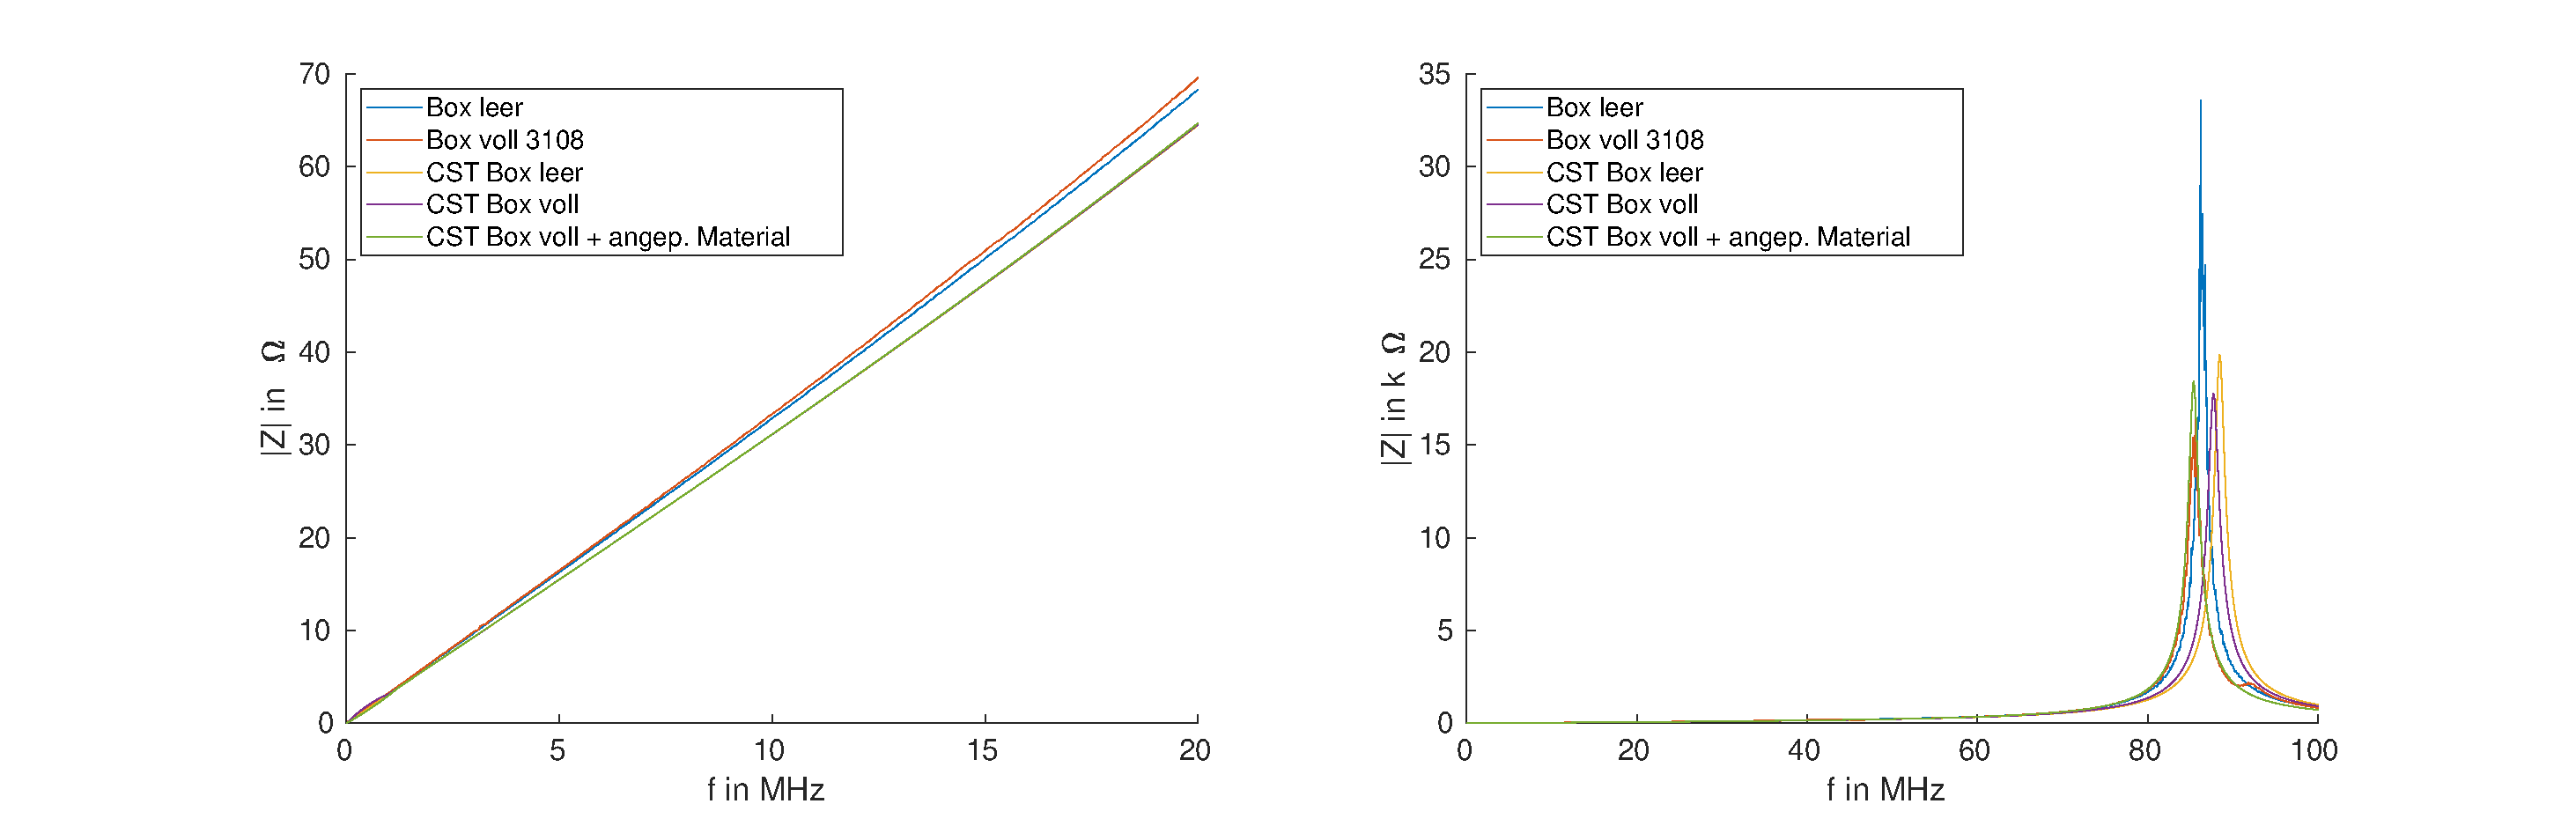
\includegraphics[width=\textwidth]{measurement_simulation_emptybox}
	\caption{Gegen\"uberstellung der Simulation der Box mit Halterung aus Kreuz und Polygon zur entsprechenden Messung.}
	\label{fig:boxpolycross}
\end{figure}
\par
Als n\"achstes in das Modell mit eingesetztem Ringkern zu evalieren. Dazu wird der Ringkern f\"ur die Simulation auf der Position um den Trovidur Ring gelegt, um die reale Box genau abzubilden. Der Aufbau ist in Abbildung~\ref{fig:RKFeRingCST} gezeigt worden. Auch hierbei wird wieder die gemessene Impedanz an der Einkopplung direkt mit der Impedanz aus der Simulation gegen\"ubergestellt. Diese Auswertung ist in Abbildung~\ref{fig:boxpolycrossrk} zu sehen.

\todo[inline,color=red!30]{Plot einf\"ugen}   

\par
Die Gegen\"uberstellung wird f\"ur alle in Abschnitt~\ref{sec:testbox} genannten Kurzschlussanordnungen in gleicher Form durchgef\"uhrt.

\par
Es zeigt sich schnell, dass insbesondere im niedrigen Frequenzbereich eine sehr geringe Abweichung zu erkennen ist. Die Mittlere Abweichung zwischen Simulation und Messung liegt unterhalb von $\SI{20}{\mega\hertz}$ bei nur \todo[inline,color=red!30]{wert und ggf Rechnung einf\"ugen}.   


\section{Auswertung der Kurzschlussanordnungen}
Nachdem die Messungen, sowie die Simulationen gegeneinander abgeglichen sind, kann die Auswertung der Kurzschlussversuche begonnen werden. Dazu wird nur die reine Ringkernimpedanz r\"uckgerechnet. Analog zum in Abschnitt~\ref{sec:ringkern} beschriebenen vorgehen, wird auch hierzu die Impedanz $Z_{rk}$ aus der gemessenen Impedanz $Z_{ges}$ nach Gleichung~\ref{eq:Zrk} herausgerechnet. Somit l\"asst sich isoliert betrachten, welcher Anteil der Ringkernimpedanz nach dem zuf\"ugen der Kurzschl\"usse noch als Rest verbleibt. Gegen\"ubergestellt werden dazu die in Unterkapitel~\ref{sec:shorts} angef\"uhrten Variationsparameter.
\par
Die maximale realtive Abweichung $a_{max}$ wird f\"ur einen Variationsparameter  nach Gleichung~\ref{eq:maxdiff} berechnet.
\begin{equation}
	\frac{Z_{max}(f) - Z_{min}(f)}{Z_{rk}(f)} = a_{max}(f)
	\label{eq:maxdiff}
\end{equation}
\par
Dabei entspricht $Z_{max}$ der h\"ochsten gemessenen Impedanz unter \"Anderung des Variationsparameters und $Z_{min}$ der niedrigsten. $Z_{rk}$ bezeichnet die Impedanz des Rinkerns ohne Kurzschl\"usse. Um die relative Abweichung $a_{percent}$ in Prozent zu erhalten, wird die relative Abweichung $a_{max}E$ nach Gleichung~\ref{eq:maxdiffpercent} mit 100 multipliziert.
\begin{equation}
	\frac{Z_{max}(f) - Z_{min}(f)}{Z_{rk}(f)}\cdot 100 = a_{percent}(f)
	\label{eq:maxdiffpercent}
\end{equation}


\subsection{Anzahl der Kurzschl\"usse}
Um den Einfluss verschiedener Anzahlen an Kurzschl\"ussen zu analysieren werden ein bis acht identische Kurzschl\"usse in der Testbox montiert. Abbildung~\ref{fig:ringcorenumberCST} zeigt die Positionen der montierten Kurzschl\"usse.
\begin{figure}[htb]
	\centering
	\subfloat{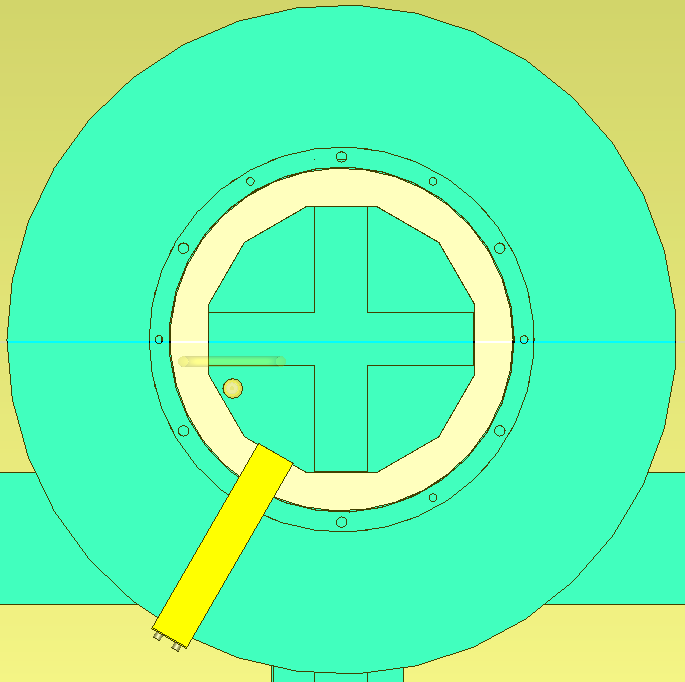
\includegraphics[height=0.24\textwidth]{1ksb30}}
	\hspace{0.0065\textwidth}
	\subfloat{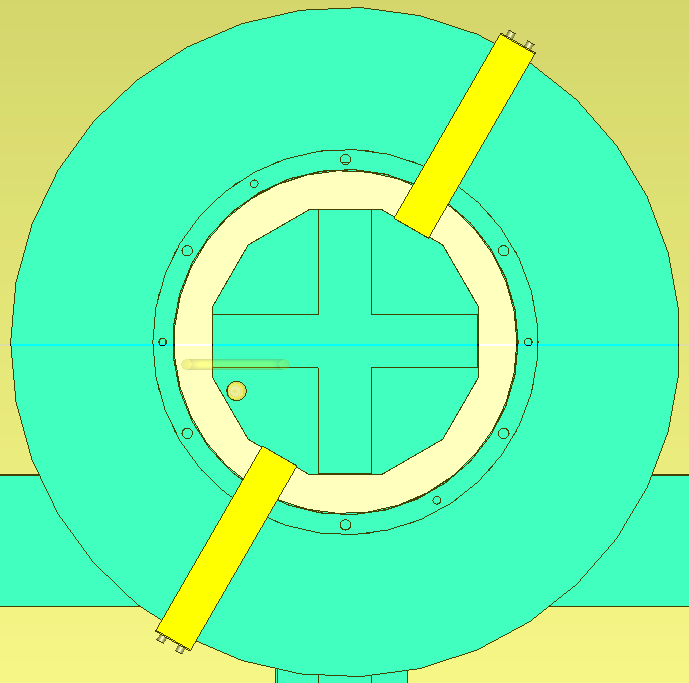
\includegraphics[height=0.24\textwidth]{2ksb30}}
	\hspace{0.0065\textwidth}
	\subfloat{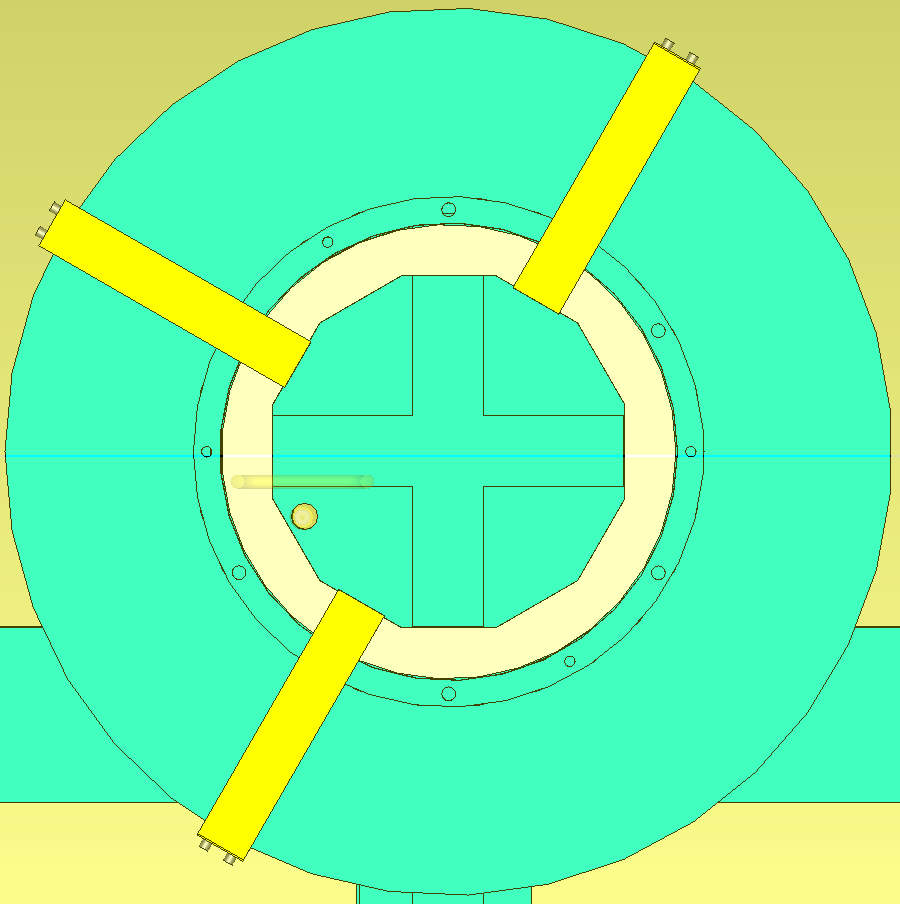
\includegraphics[height=0.24\textwidth]{3ksb30}}
	\hspace{0.0065\textwidth}
	\subfloat{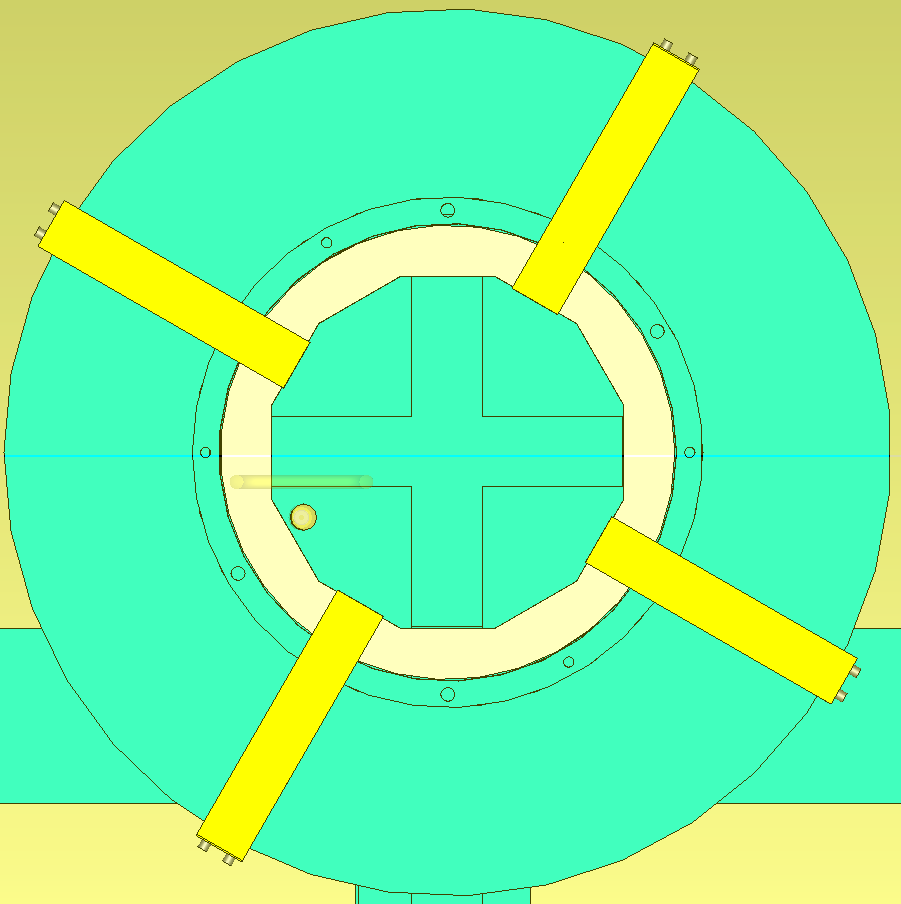
\includegraphics[height=0.24\textwidth]{4ksb30}}
	\\
	\subfloat{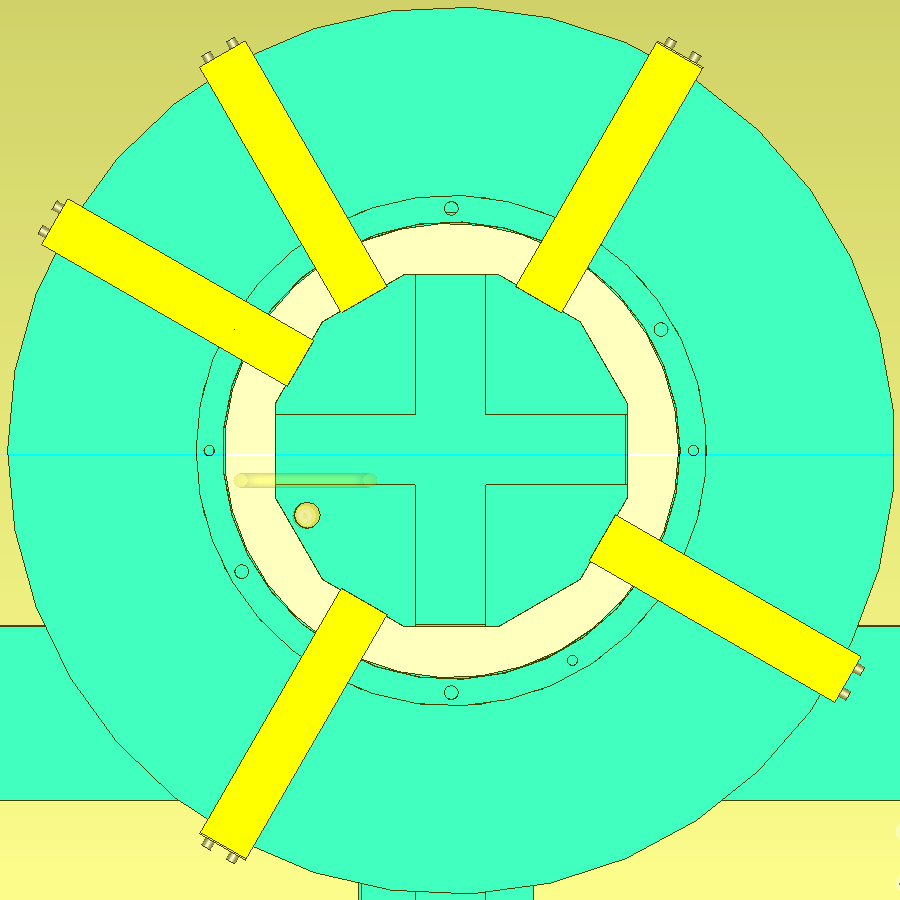
\includegraphics[height=0.24\textwidth]{5ksb30}}
	\hspace{0.0065\textwidth}
	\subfloat{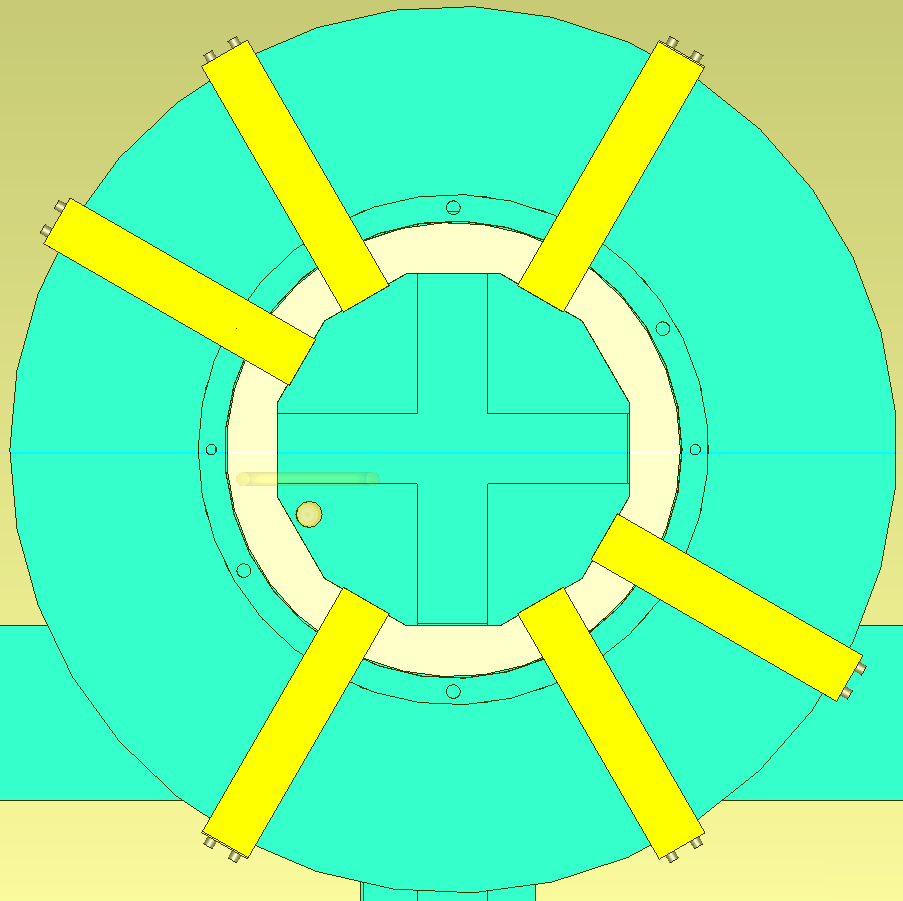
\includegraphics[height=0.24\textwidth]{6ksb30}}
	\hspace{0.0065\textwidth}
	\subfloat{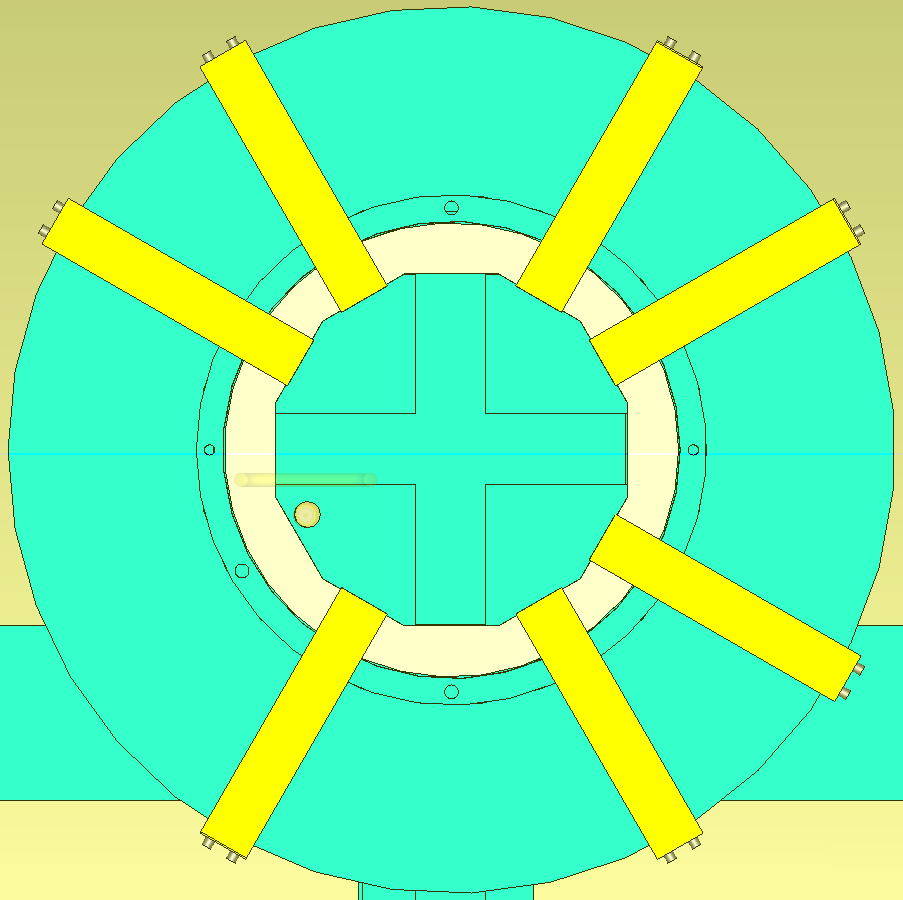
\includegraphics[height=0.24\textwidth]{7ksb30}}
	\hspace{0.0065\textwidth}
	\subfloat{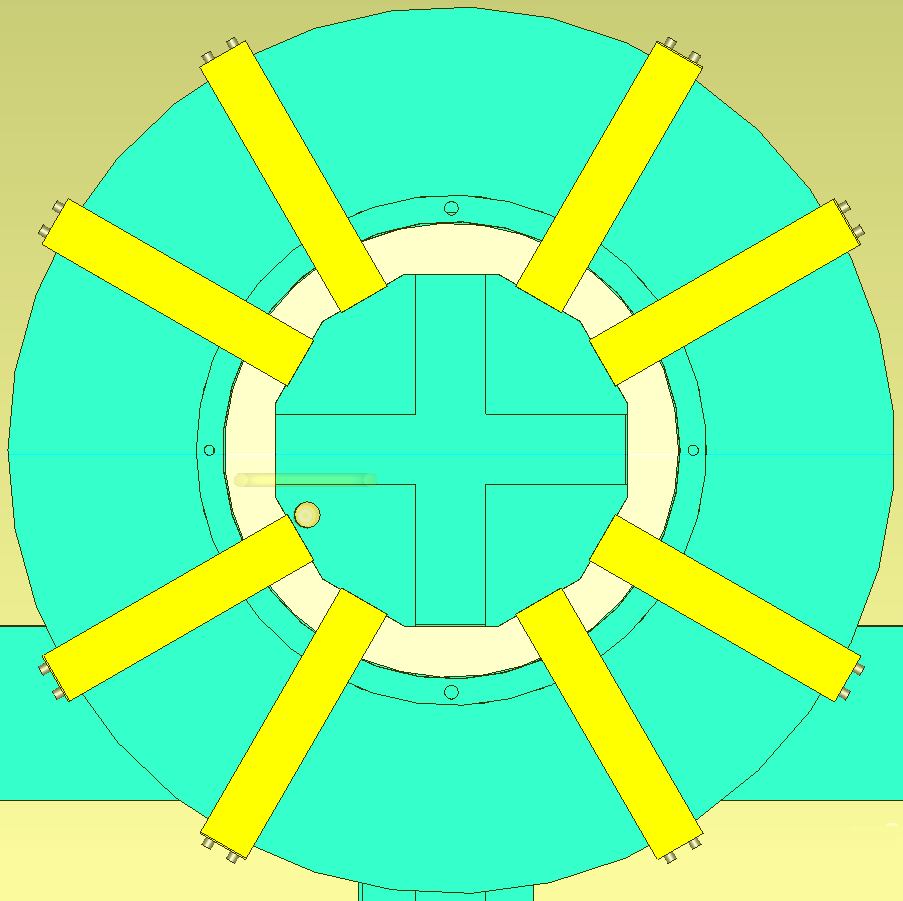
\includegraphics[height=0.24\textwidth]{8ksb30}}
	\caption{Unterschiedliche Anzahlen an montierten Kurzschl\"ussen an verschiedenen Positionen.}
	\label{fig:ringcorenumberCST}
\end{figure}
\par
% \todo[inline,color=red!30]{Erkl\"aren warum 8KS bei der Auswertung nicht mehr auftaucht}  
Die achte Kurzschlusschiene, welche in Grafik~\ref{fig:ringcorenumberCST} zu sehen ist, konnte bei der endg\"ultigen Auswertung nicht ber\"ucksichtigt werden. Dieser Kurzschluss liegt sehr nah am Einkopplungsrohr, sodass ein direkter Kontakt dazu besteht. F\"ugt man einen Abstandshalter aus Schaumstoff zu, so wird das die Einkopplung etwas nach oben gebogen. Die Messung liefert daher verf\"alschte Ergebnisse. F\"ur die endg\"ultige Auswertung wurden folglich nur 1-7 Kurzschl\"usse betrachtet.
\begin{figure}[htb]
	\centering
	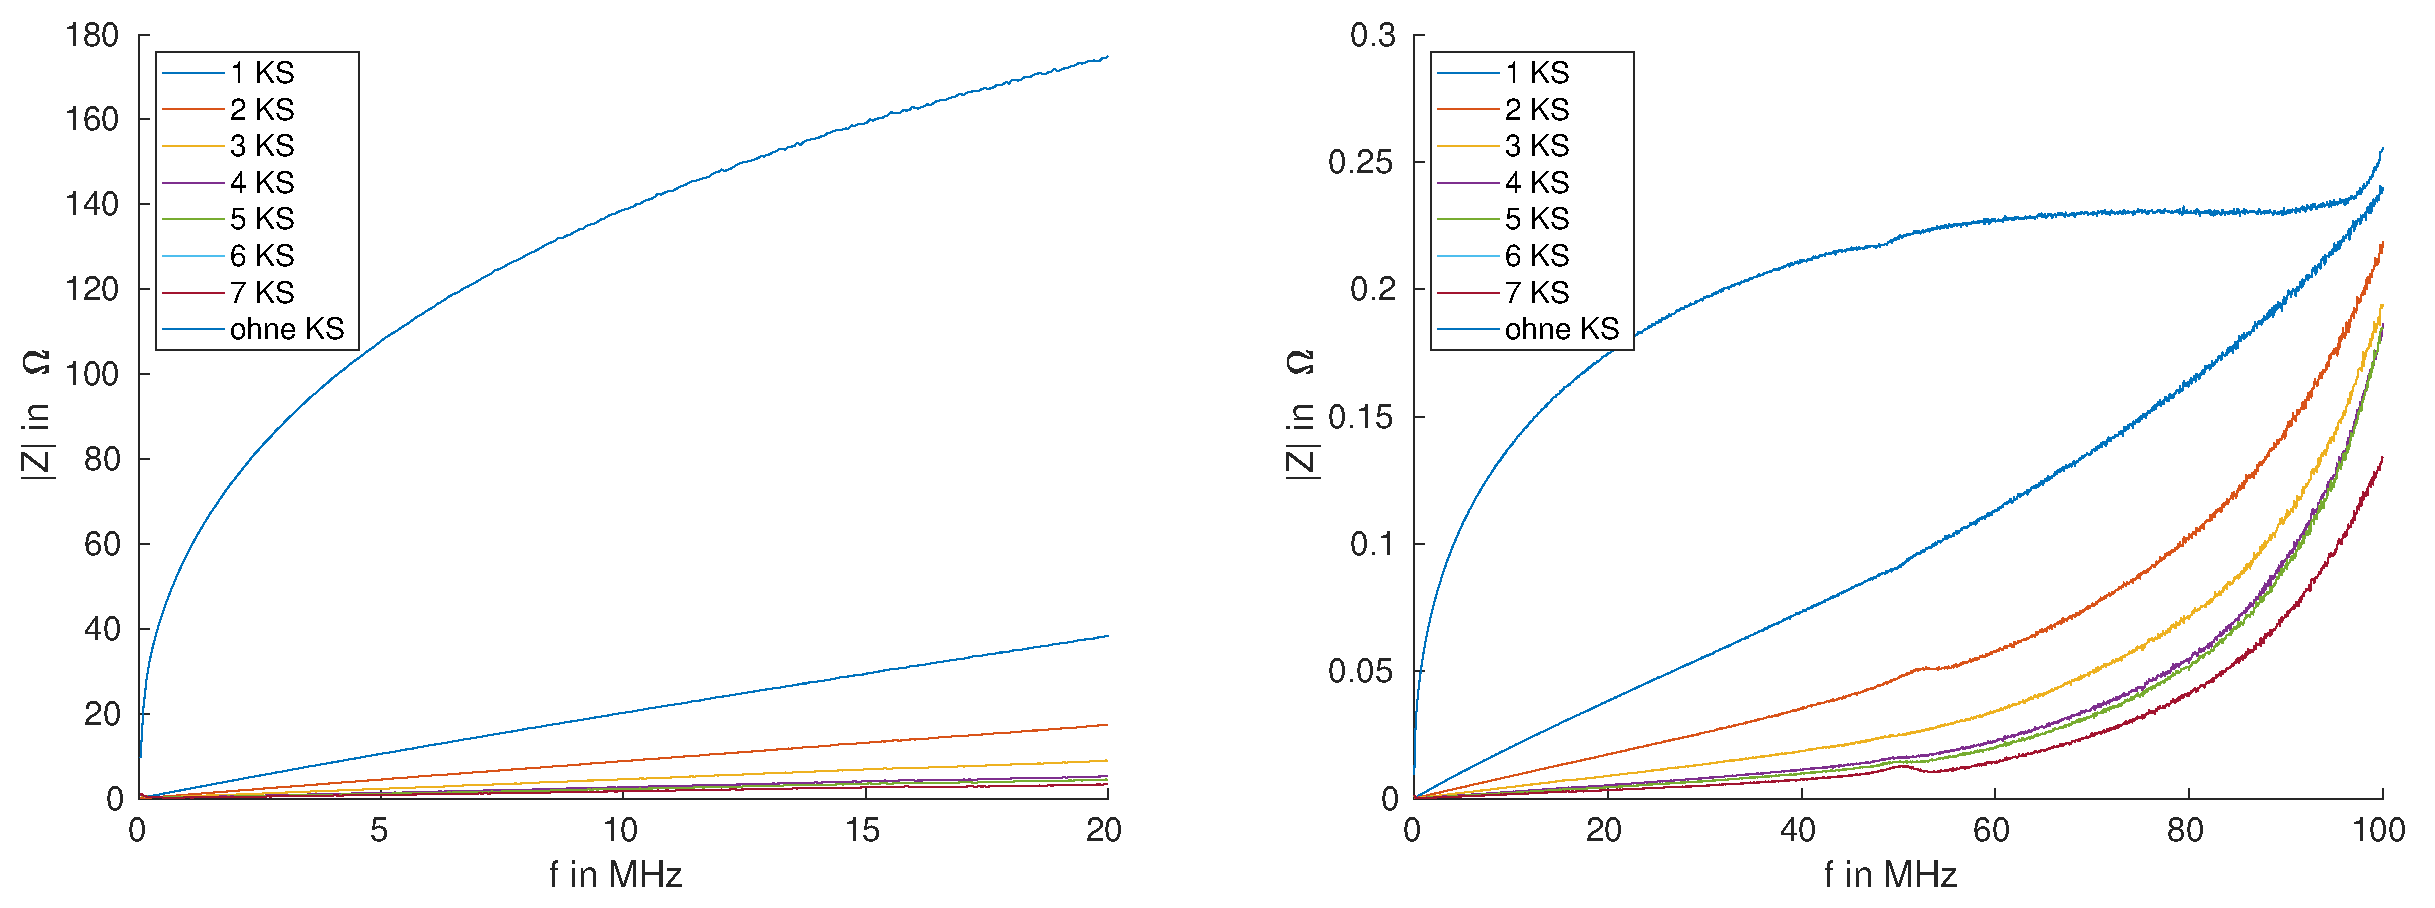
\includegraphics[width=\textwidth]{impedance_numberKS_ringcore}
	\caption{Gegen\"uberstellung der Ringkernimpedanz f\"ur verschiedene Anzahlen an Kurzschl\"ussen}
	\label{fig:ringcorenumber}
\end{figure}
\par
Es f\"allt auf, dass der gr\"o\ss{}te Sprung zwischen null und einem Kurzschluss liegt. Das bedeutet, dass die Montage weiterer Kurzschl\"usse mit zunehmender Anzahl weniger effektiv ist. Um das zu verdeutlichen wird eine weitere Gegen\"uberstellung angesetzt, bei der eine bestimmte Frequenz fixiert wird, und die Impedanz $Z_{rk}$ \"uber der Anzahl an Kurzschl\"ussen aufgetragen ist. Die Fixierten Frequenzen liegen dabei bei 5, 10 und $\SI{20}{\mega\hertz}$, da insbesondere der niedrigere Frequenzbereich f\"ur den Beschleunigerbetrieb von Relevanz ist~\citep{frey2015status}. Die Gegen\"uberstellung ist in Abbildung~\ref{fig:ringcorenumber20} aufgetragen.
\begin{figure}[htb]
	\centering
	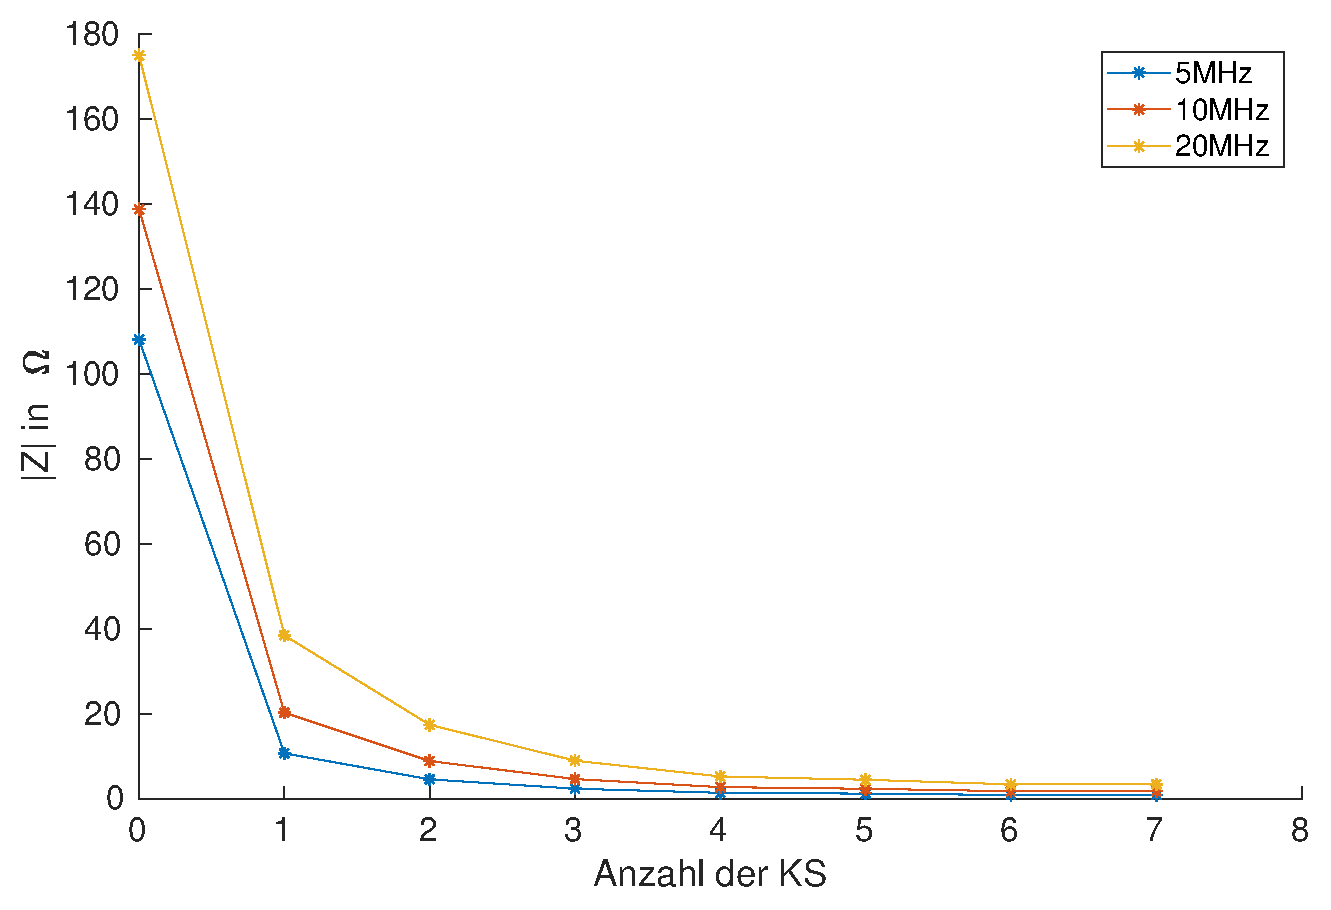
\includegraphics[width=0.5\textwidth]{RK_Impedanz_numberKS_frequenz}
	\caption{Gegen\"uberstellung der Ringkernimpedanz mit verschiedenen Anzahlen an Kurzschl\"ussen bei 5, 10 und $\SI{20}{\mega\hertz}$.}
	\label{fig:ringcorenumber20}
\end{figure}
\par
Der Effekt der Kurzschl\"usse wird mittels Gleichung~\ref{eq:maxdiffpercent} errechnet. Wird $Z_{max}$ auf den Wert $Z_{rk}(\SI{20}{\mega\hertz})$ gesetzt, also den Fall ohne Kurzschl\"usse und $Z_{min}$ auf $Z_{1KS}(\SI{20}{\mega\hertz})$, so ergibt sich eine prozentuale Abweichung nach Gleichung~\ref{eq:maxdiffpercentzeroone}.
\begin{equation}
	\frac{\SI{175,1145}{\Omega} - \SI{38,4525}{\Omega}}{\SI{175,1145}{\Omega}}\cdot 100 = \SI{78,042}{\%}
	\label{eq:maxdiffpercentzeroone}
\end{equation}
\par
Das hei\ss{}t ein Kurzschluss verringert die Impedanz des Ringkerns bereits um $\SI{78,042}{\%}$ verglichen mit der Impedanz ohne Kurzschluss. Wird hingegen $Z_{max}$ auf $Z_{1KS}(\SI{20}{\mega\hertz})$ und $Z_{min}$ zu $Z_{2KS}(\SI{20}{\mega\hertz})$ gesetzt, so ergibt sich eine Abweichung nach Gleichung~\ref{eq:maxdiffpercentonetwo}.
\begin{equation}
	\frac{\SI{38,4525}{\Omega} - \SI{17,3717}{\Omega}}{SI{175,1145}{\Omega}}\cdot 100 = \SI{12,038}{\%}
	\label{eq:maxdiffpercentonetwo}
\end{equation}
\par
Die Verringerung der Impedanz f\"allt also deutlich geringer aus, als noch beim Unterschied von Null zu einem Kurzschluss. Auch der Vergleich von einem zu sieben Kurzschl\"ussen, also mit $Z_{max}$ gleich $Z_{1KS}(\SI{20}{\mega\hertz})$ und $Z_{min}$ gleich $Z_{7KS}(\SI{20}{\mega\hertz})$ f\"allt mit der Abweichung nach Gleichung~\ref{eq:maxdiffpercentoneseven}
\begin{equation}
	\frac{\SI{38,4525}{\Omega} - \SI{3,3453}{\Omega}}{SI{175,1145}{\Omega}}\cdot 100 = \SI{20,048}{\%}
	\label{eq:maxdiffpercentoneseven}
\end{equation}
\par
vergleichsweise gering aus. Je nach Anforderung ist also zu \"uberlegen, ob ein Kurzschluss bereits eine ausreichende Reduktion erzeugt. Das ist insbesondere beim Einbau in die Kavit\"at von Relevanz, da eine Montage mehrerer Kurzschl\"usse einen nicht unerheblichen Aufwand mit sich zieht. 


\subsection{Breite der Kurzschl\"usse}
Die Breite der Kurzschl\"usse ist ein Parameter, welcher durch die Schienenartige Form der Kurzschl\"usse leicht zu variieren ist, da diese nur aus einem Blech geschnitten werden. Die Montierten Kurzschl\"usse verschiedener Breiten sind in Abbildung~\ref{fig:ringcorewidthCST} abgebildet.
\begin{figure}[htb]
	\centering.
	\subfloat[$\SI{20}{\milli\meter}$]{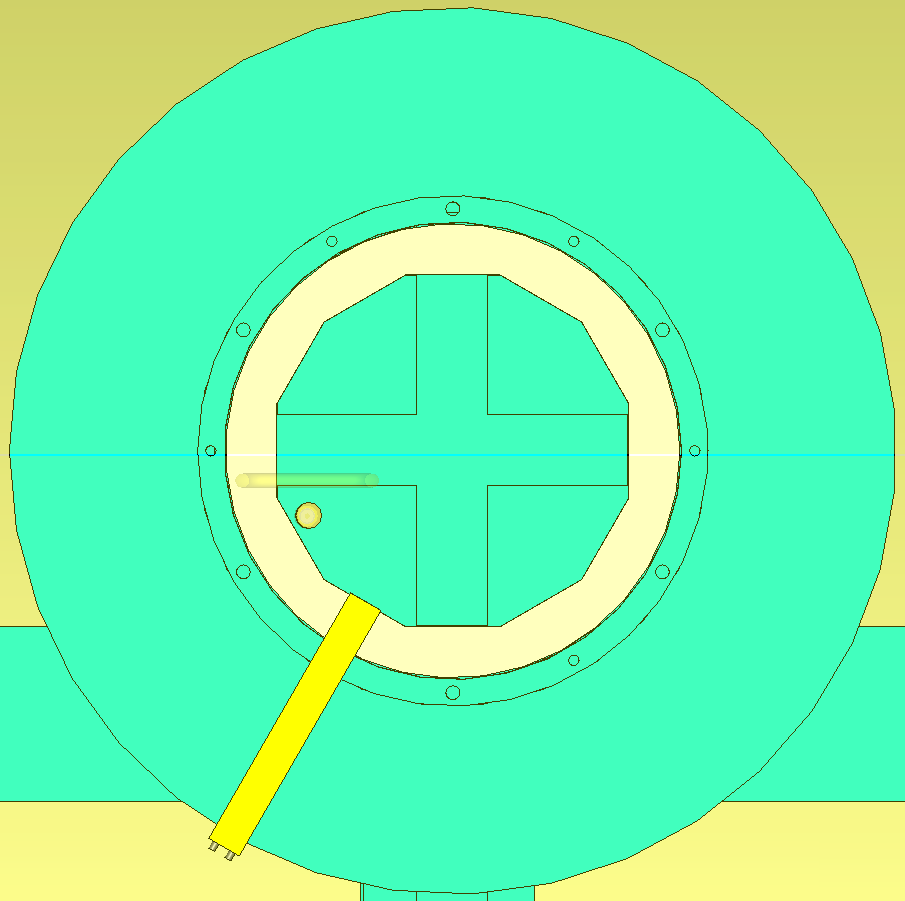
\includegraphics[height=0.3\textwidth]{1ksb20}}
	\hspace{0.02\textwidth}
	\subfloat[$\SI{30}{\milli\meter}$]{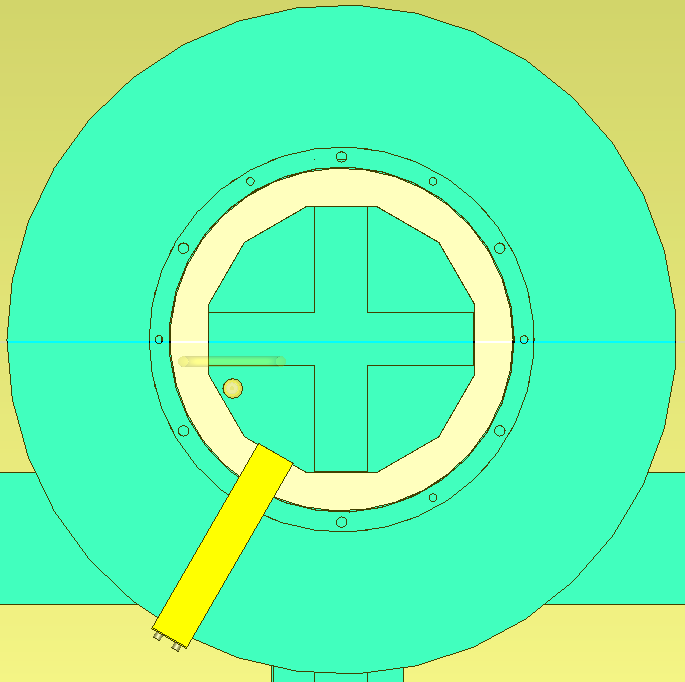
\includegraphics[height=0.3\textwidth]{1ksb30}}
	\hspace{0.02\textwidth}
	\subfloat[$\SI{50}{\milli\meter}$]{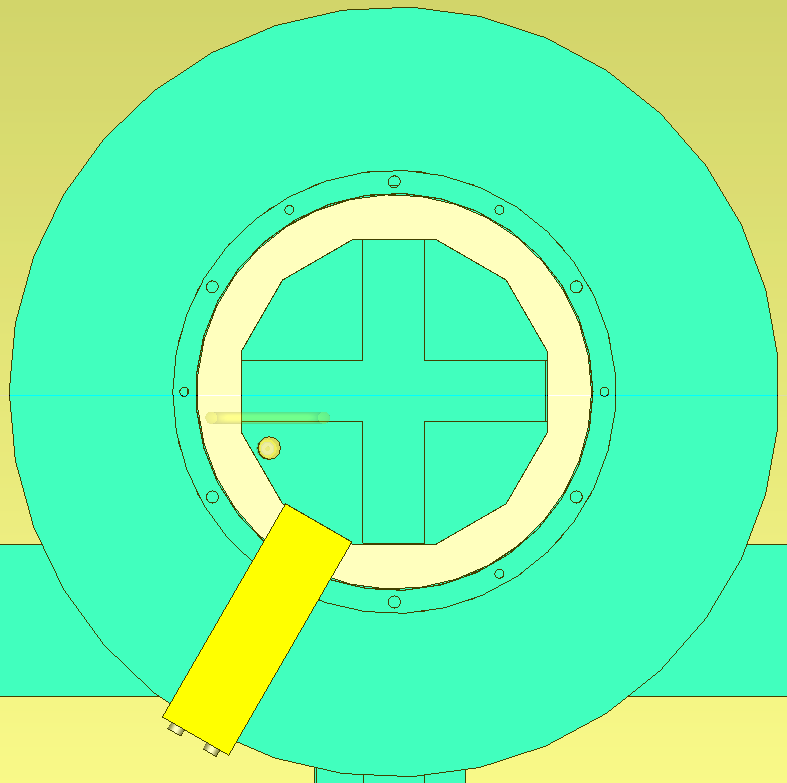
\includegraphics[height=0.3\textwidth]{1ksb50}}
	\caption{Jeweils ein montierter Kurzschluss mit verschiedenen Breiten.}
	\label{fig:ringcorewidthCST}
\end{figure}
\par
Da eine h\"ohere Anzahl an Kurzschl\"ussen eine verringerte Ringkernimpedanz als Ergebnis liefert, liegt die Vermutung nahe, dass auch breitere Kurzschl\"usse die Ringkernimpedanz weiter verringern k\"onnen. Die Gegen\"uberstellung der Ringkernimpedanz $Z_{rk}$ ist in Abbildung~\ref{fig:ringcorewidth} zu sehen.
\begin{figure}[htb]
	\centering
	\subfloat[1 Kurzschluss]{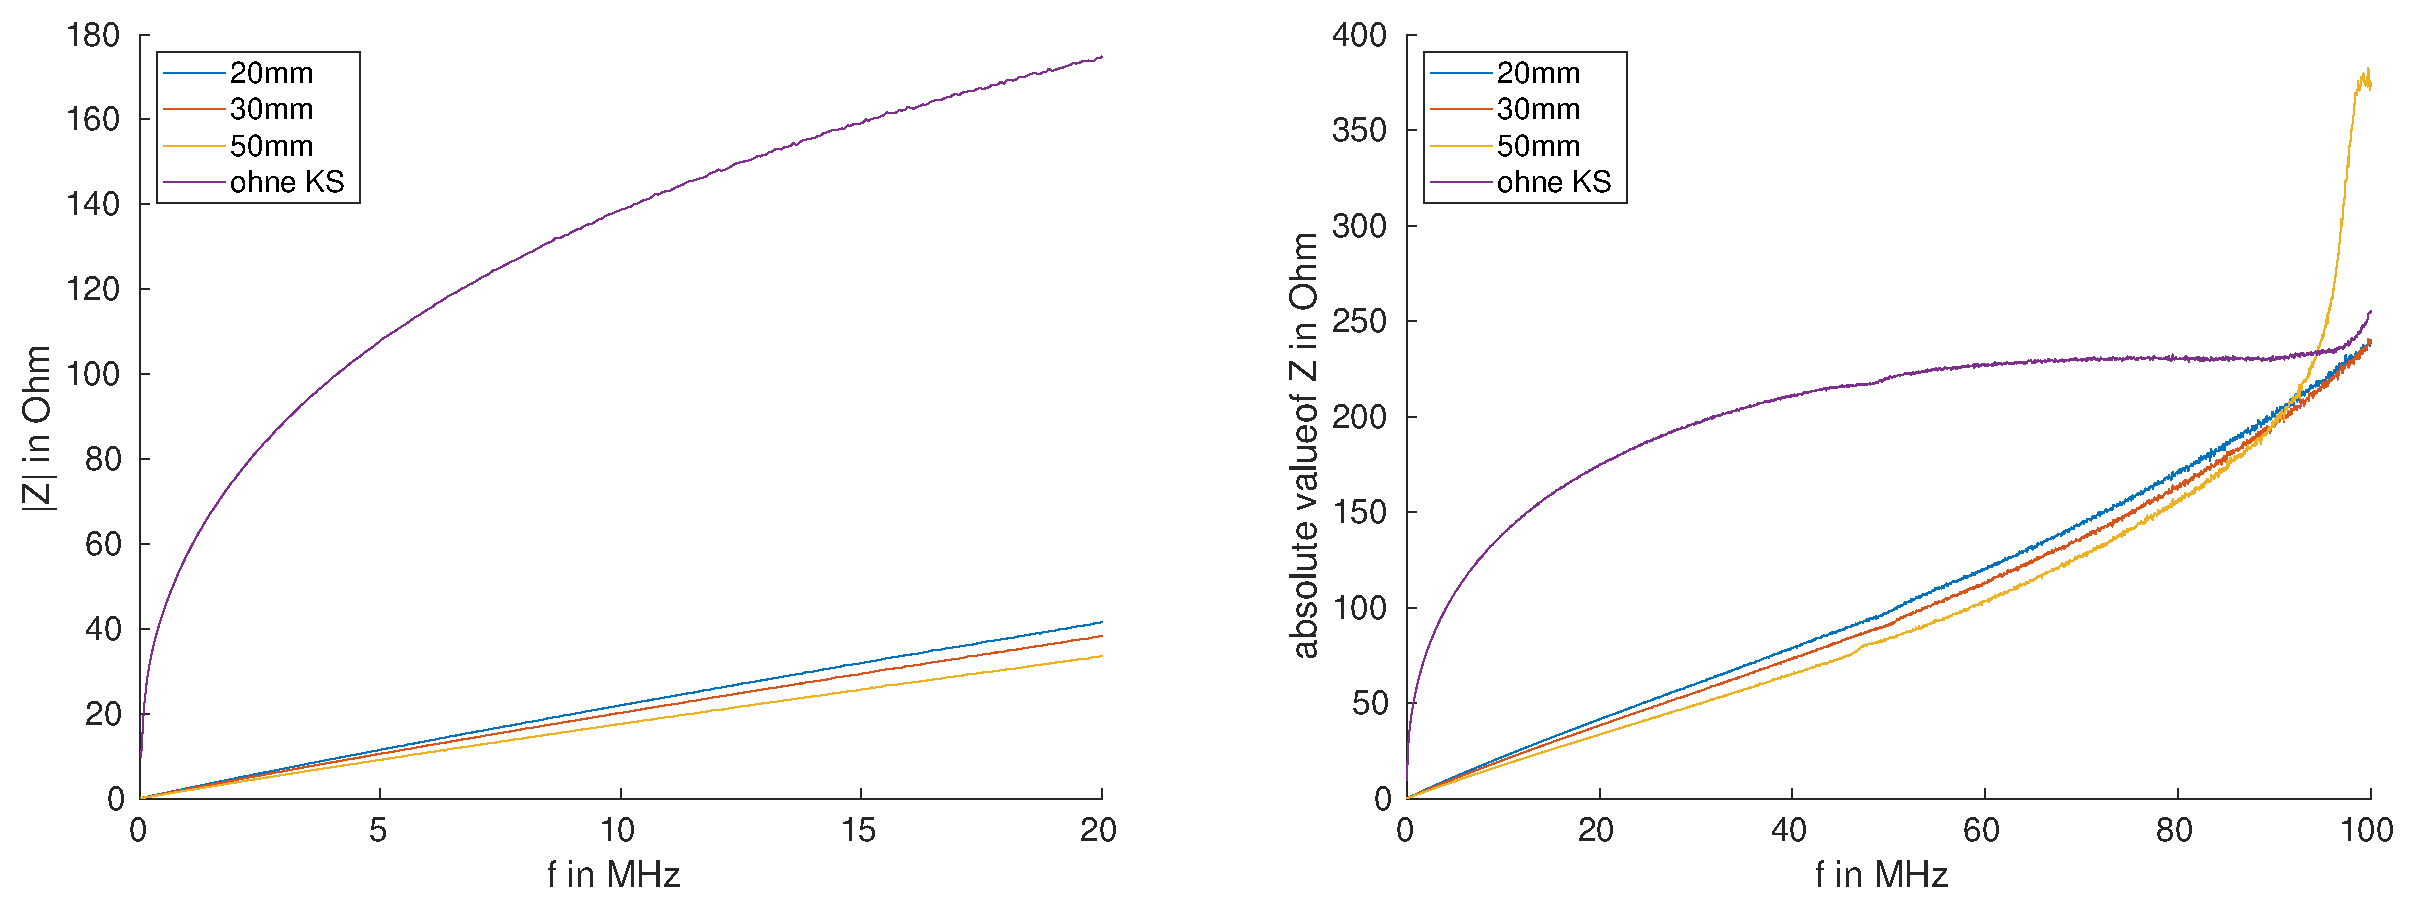
\includegraphics[width=\textwidth]{Z_RK_width_1KS}}
	\\
	\subfloat[2 Kurzschl\"usse]{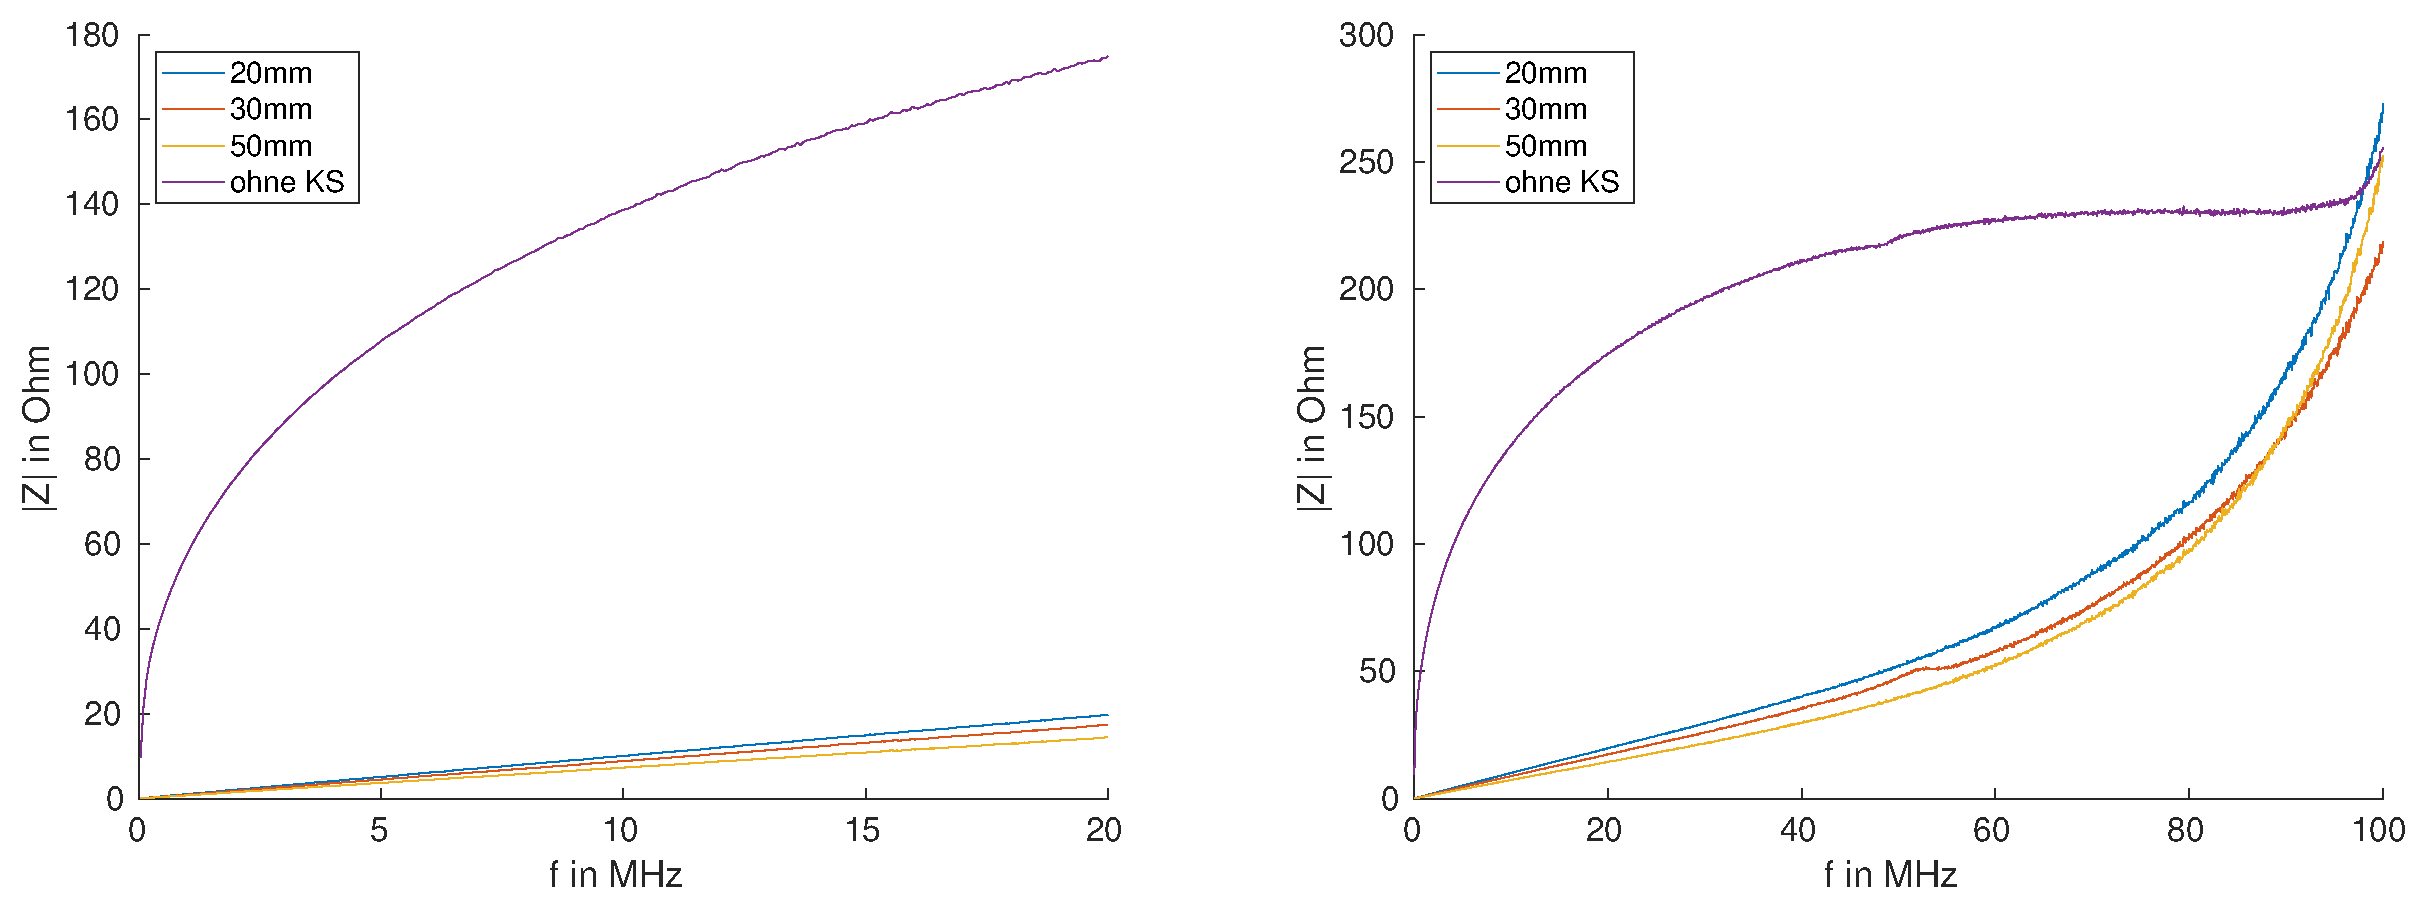
\includegraphics[width=\textwidth]{Z_RK_width_2KS}}
	\caption{Gegen\"uberstellung der Ringkernimpedanz f\"ur verschiedene Breiten der Kurzschl\"usse.}
	\label{fig:ringcorewidth}
\end{figure}
\par
Auch hier wird wieder ein genaueres Augenmerk auf den relevanten Frequenzbereich unterhalb von $\SI{20}{\mega\hertz}$ gelegt. Dazu werden die Frequenzen von 5, 10 und $\SI{20}{\mega\hertz}$ geplottet und jeweils die verschiedenen Breiten gegen\"ubergestellt. Abbildung~\ref{fig:ringcorewidth20} zeigt die genannte Gegen\"uberstellung.
\begin{figure}[htb]
	\centering
	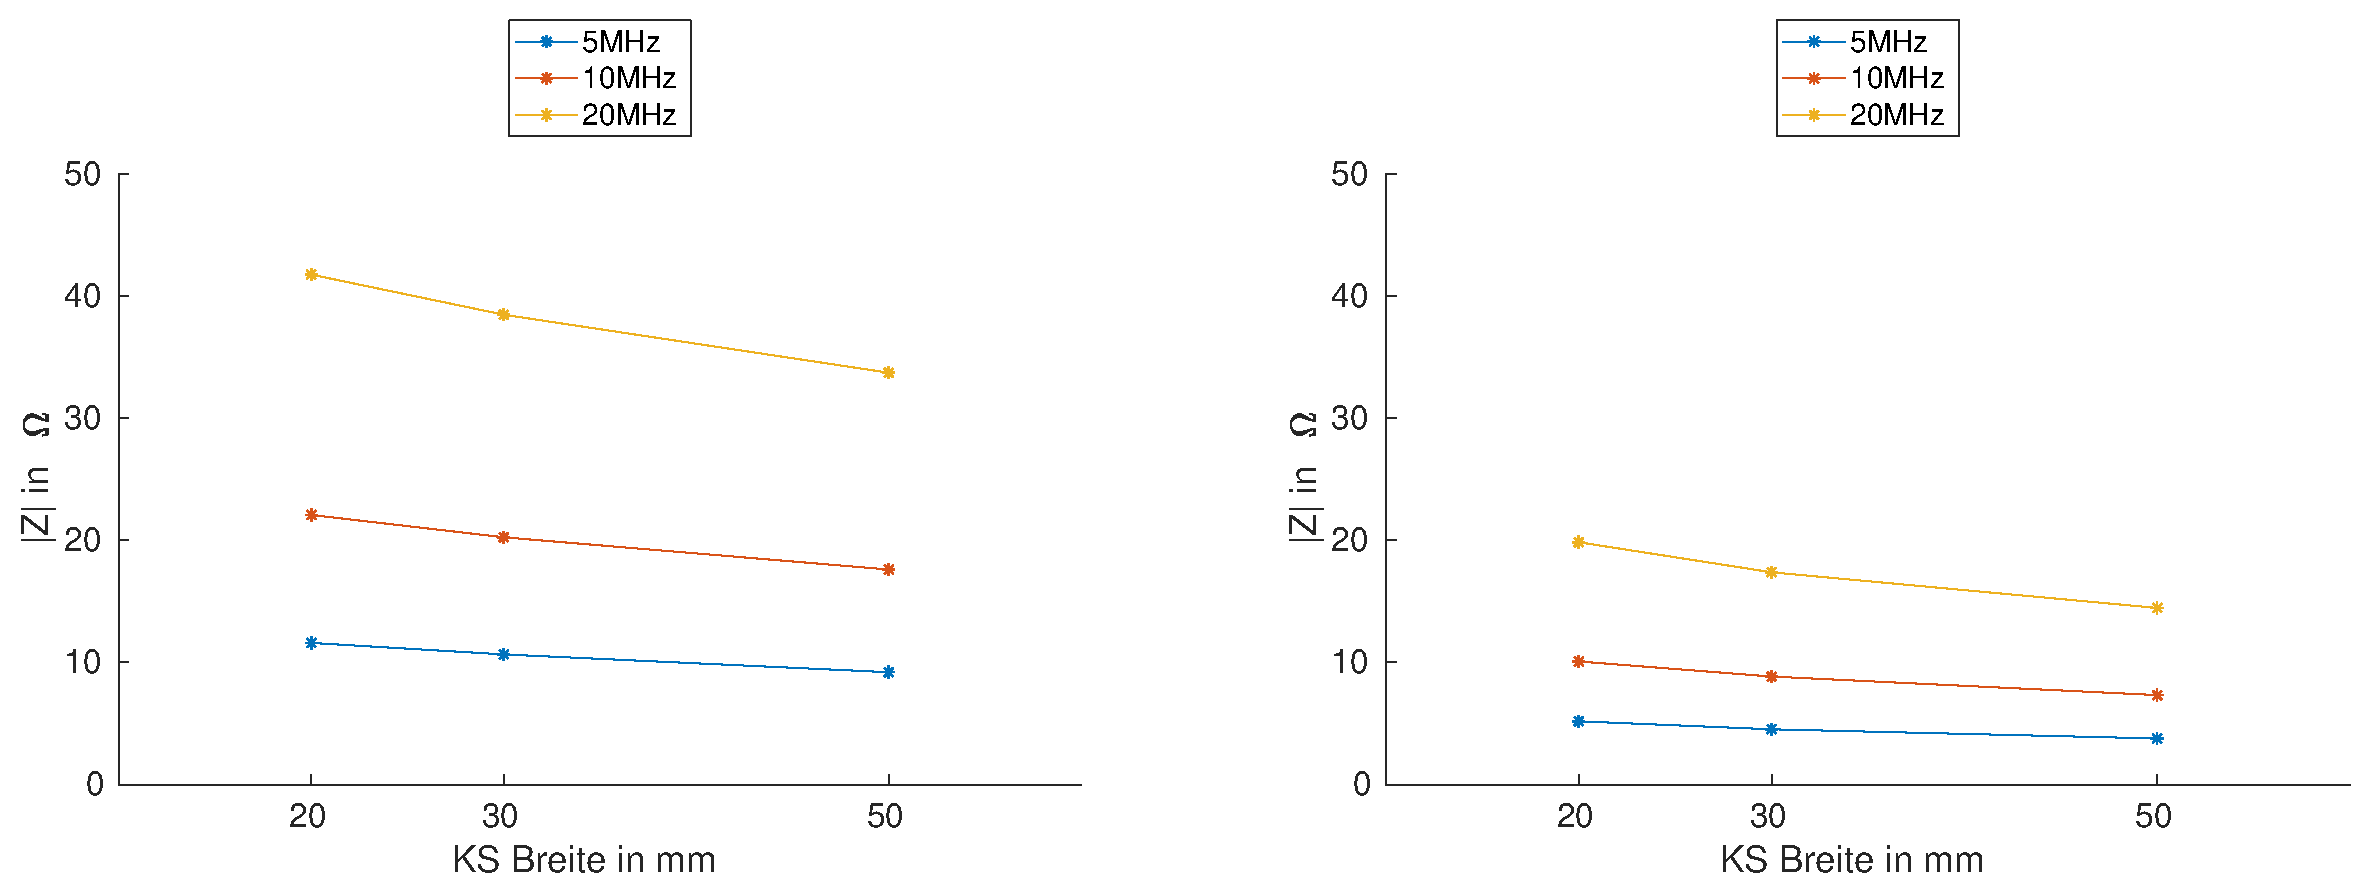
\includegraphics[width=\textwidth]{RK_Impedanz_width_frequenz}
	\caption{Gegen\"uberstellung der Ringkernimpedanz bei 5, 10 und $\SI{20}{\mega\hertz}$. Links: 1KS, rechts: 2KS.}
	\label{fig:ringcorewidth20}
\end{figure}
\par
Das Ergebnis zeigt, dass ein breiterer Kurzschluss das Ergebnis der resultierenden Ringkernimpedanz weiter verringert. Diese Variation liefert im Extremfall, also dem Unterschied von $\SI{20}{\milli\meter}$ zu $\SI{50}{\milli\meter}$ bei einer Anzahl von zwei Kurzschl\"ussen und einer Frequenz von $\SI{20}{\mega\hertz}$, eine Verringerung der Ringkernimpedanz nach Gleichung~\ref{eq:maxdiffpercent} von rund $\SI{2,8}{\%}$. Das bedeutet, dass die Breite der Kurzschl\"usse wesentlich weniger Auswirkungen auf die resultierende Ringkernimpedanz hat, wie die Anzahl an Kurzschl\"ussen. Besonders deutlich wird das im Vergleich zwischen einem Kurzschluss der Breite $\SI{50}{\milli\meter}$ mit zwei Kurzschl\"ussen der Breite $\SI{20}{\milli\meter}$. Trotz des geringeren Platzbedarfs, liefern die zwei schmalen Kurzschl\"usse eine deutlich geringere Impedanz.  Sollte aus Platzgr\"unden eine Montage Breiterer Kurzschl\"usse in der Kavit\"at zu Problemen f\"uhren, so ist eine h\"ohere Anzahl von schmaleren Kurzschl\"ussen vorzuziehen. 


\subsection{L\"ange der Kurzschl\"usse}
\begin{figure}[htb]
	\centering
	\subfloat[$\SI{160}{\milli\meter}$]{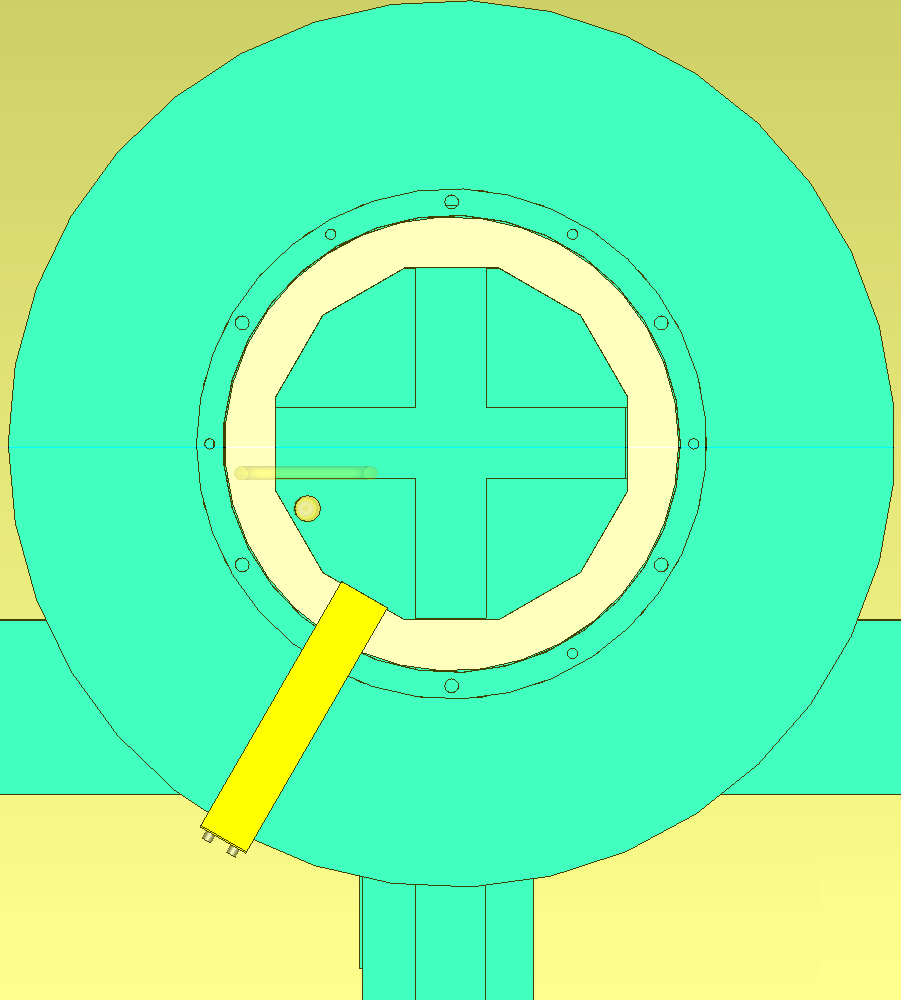
\includegraphics[height=0.3\textwidth]{1ksh160}}
	\hspace{0.05\textwidth}
	\subfloat[$\SI{200}{\milli\meter}$]{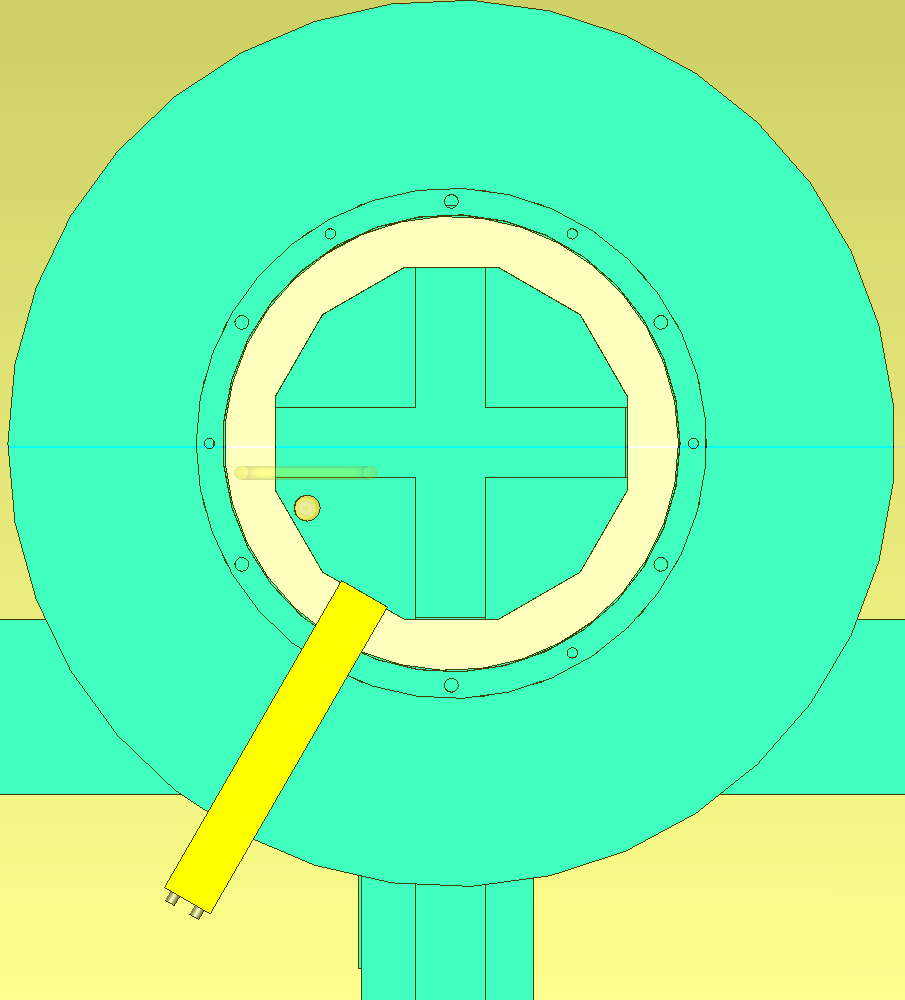
\includegraphics[height=0.3\textwidth]{1ksh200}}
	\hspace{0.05\textwidth}
	\subfloat[$\SI{250}{\milli\meter}$]{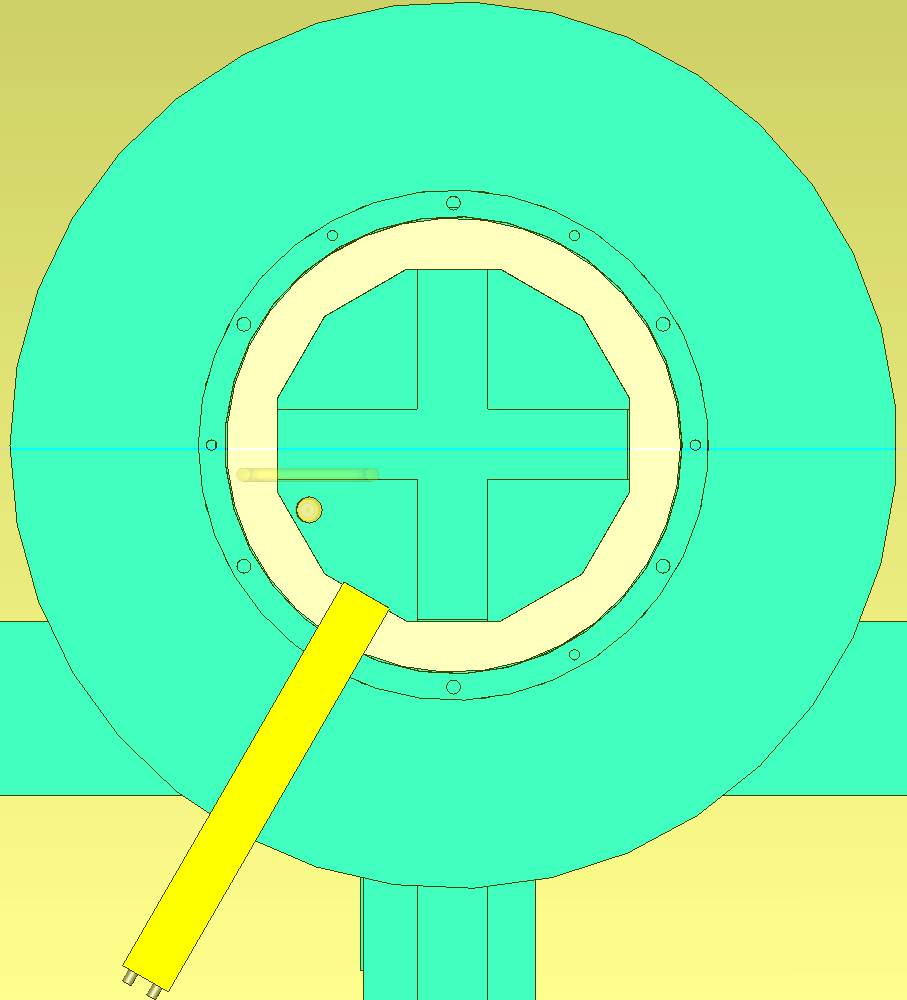
\includegraphics[height=0.3\textwidth]{1ksh250}}
	\caption{Jeweils ein montierter Kurzschluss mit verschiedenen L\"angen.}
	\label{fig:ringcoreheigthCST}
\end{figure}


\subsection{Dicke der Kurzschl\"usse}

\begin{figure}[htb]
	\centering
	\subfloat[1 Kurzschluss]{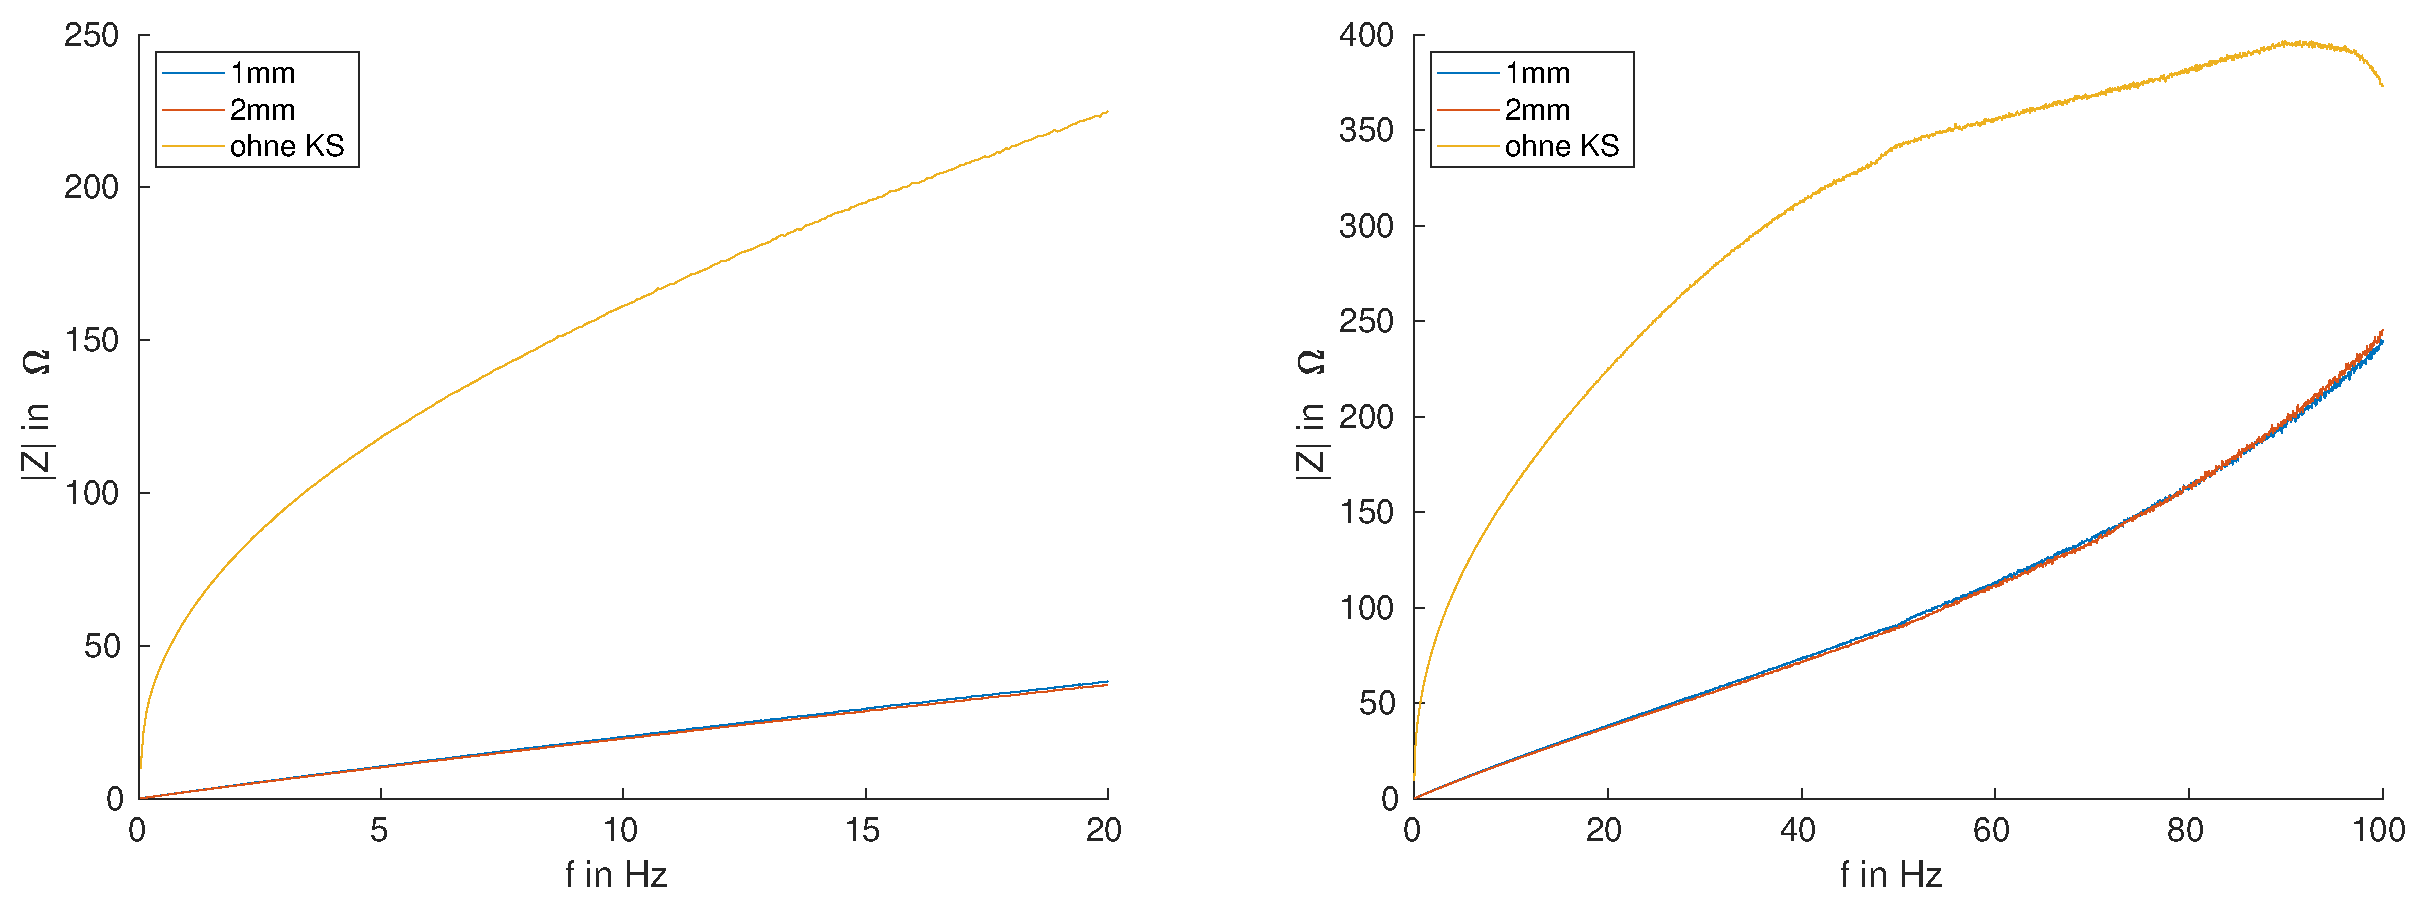
\includegraphics[width=\textwidth]{Z_RK_thick_1KS}}
	\\
	\subfloat[2 Kurzschl\"usse]{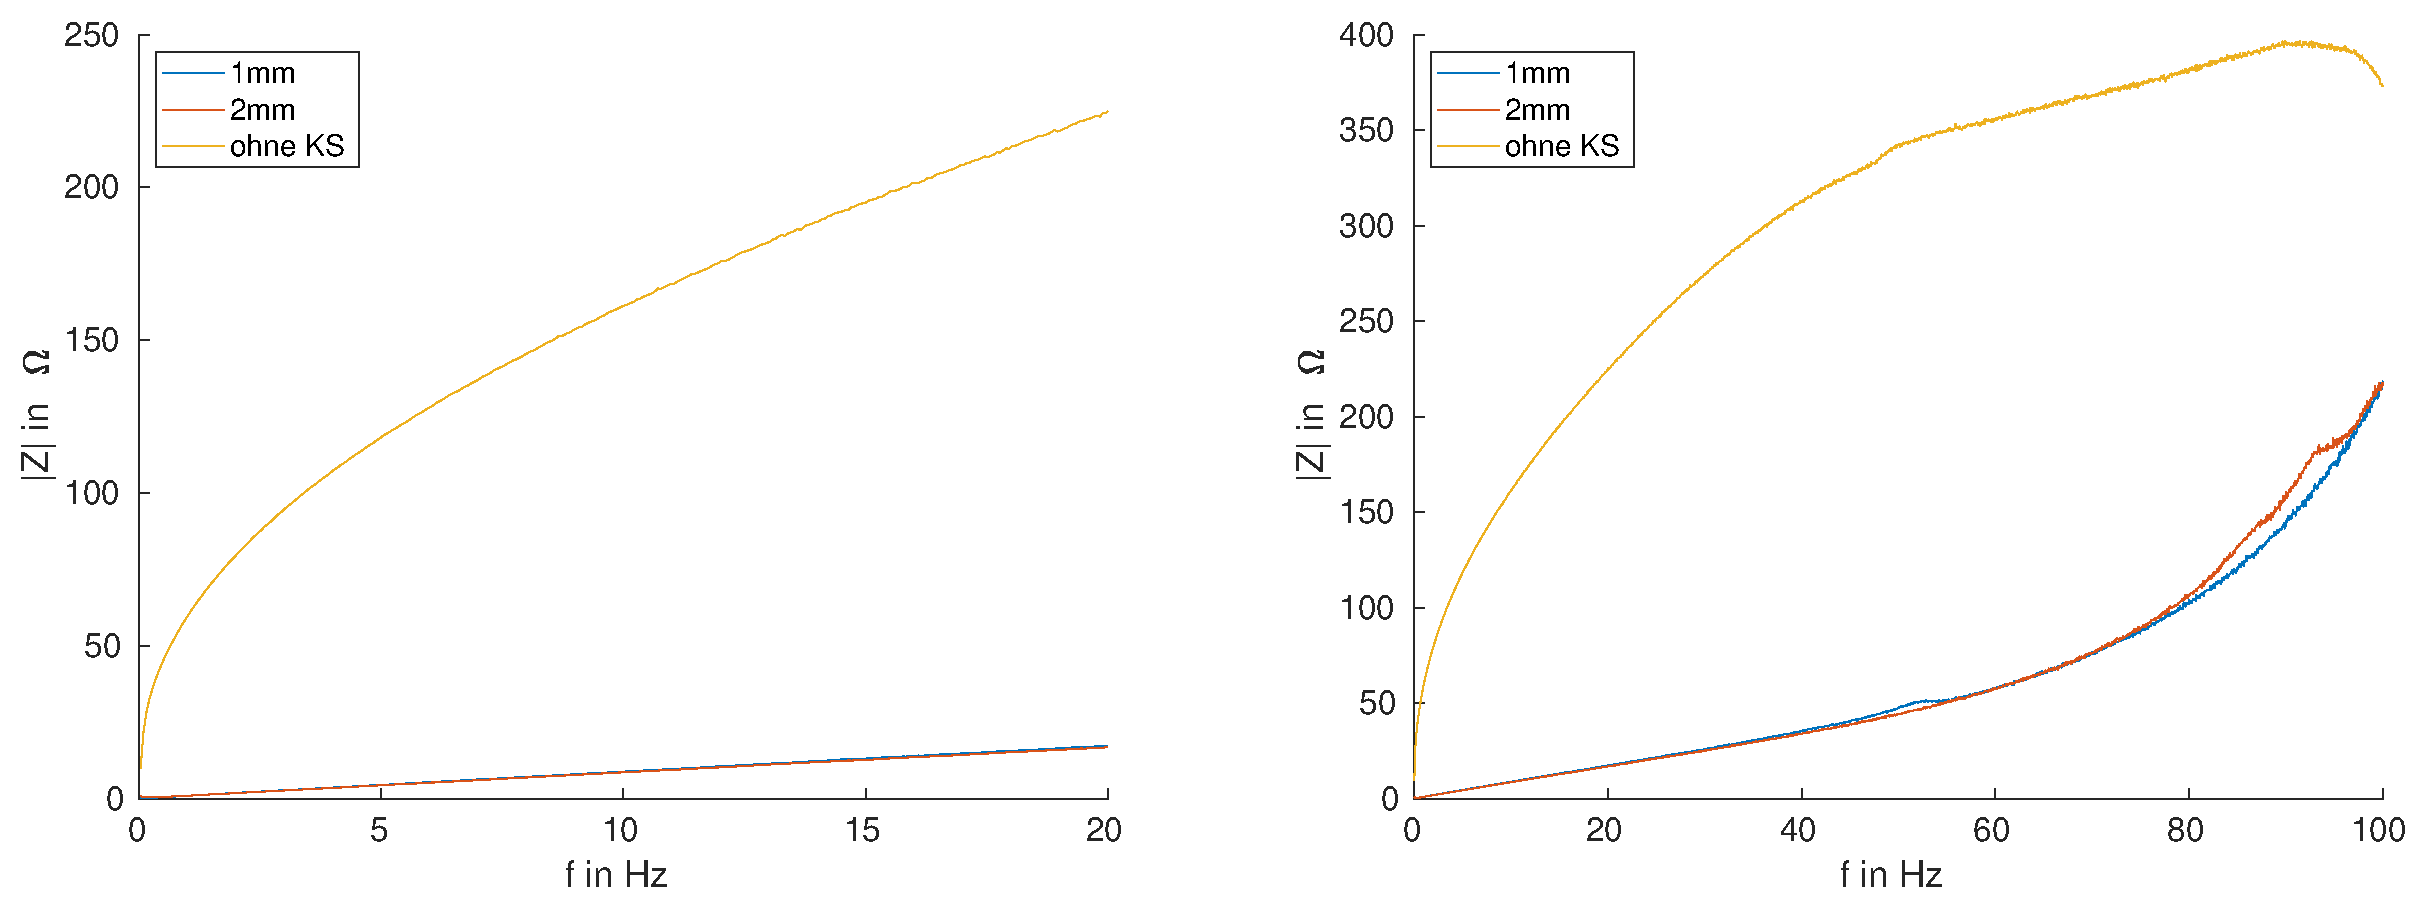
\includegraphics[width=\textwidth]{Z_RK_thick_2KS}}
	\caption{Gegen\"uberstellung der Ringkernimpedanz f\"ur verschiedene Dicken der Kurzschl\"usse.}
	\label{fig:ringcorethick}
\end{figure}